The study described in Section \ref{sec:emp} evidences the challenge of managing MBT suites during software evolution. To test whether distance functions can help to cope with this problem, we ran a second empirical study. The goal of this study was to analyze the use of distance functions to automatically classify changes in use case documents that could impact MBT suites. 

\subsection{Subjects and Functions}
For that, our study was also run in the context of the industrial projects SAFF and BZC. 
%that were developed in the context of a cooperation between
%our research lab and two different companies, Ingenico do Brasil Ltda and Viceri Solution Ltda. The SAFF project is an information
%system that manages reports on payment terminals,
%and BZC is a system for optimizing e-commerce logistic activities. 
It is important to remember that both projects used agile methodologies to guide the development and updates in the requirement artifacts were frequent. Moreover, their teams used both CLARET \citep{dalton2017claret}, for use case specification, and LTS-BT \citep{cartaxo2008lts} for generating MBT suites. 

%Both projects use manually executed system-level black-box test cases for regression purposes. In this sense, test case history data is very important since can help to keep track of the system evolution and to avoid functionality regression. However, the teams reported that often discard test cases when the related steps on the system use cases are updated in any form, which they refer to as a practical management problem.

As our study focuses on the use of distance functions, we selected a set of ten of the most well-known functions that have been used in different contexts: Hamming \citep{hamming1950error}, LCS \citep{han2007efficient:LCS}, Cosine \citep{huang2008similaritycosine}, Jaro \citep{de1mahalanobis:jaro}, Jaro-Winkler \citep{de1mahalanobis:jaro}, Jaccard \citep{Lu2013SimilaridadeJaccard}, Ngram \citep{Kondrak2005ngram}, Levenshtein \citep{Levenshtein_SPD66}, OSA \citep{Damerau:1964}, and Sorensen Dice \citep{sorensen1948method}. To perform systematic analyses, we normalize their results in a way that their values range from zero to one. Values near zero refer to low similarity, while near one values indicate high similarity. We reused open-source implementations of all ten functions\footnote{https://github.com/luozhouyang/python-string-similarity}\footnote{https://rosettacode.org/wiki/Category:Programming\_Tasks}. To customize and analyze the edits in the context of our study, we created our own tool and scripts that were verified through a series of tests.

%that is available on our website\footnote{Not presented due to double-blind review.}.

We mined the projects' repository and collected all use case edits. Each of these edits would then impact the test cases. We call ``impacted'' any test case that includes steps that were updated during model maintenance. However, we aim to use distance functions to help us to classify these edits and avoid the test case discard.

%\subsection{Research Questions}
To guide our investigation, we defined the following research questions:
\begin{itemize}
\item \textbf{RQ4}: Can distance functions be used to classify the impact of edits in use case documents?  
\item \textbf{RQ5}: Which distance function presents the best results for classifying edits in use case documents?
\end{itemize}

\subsection{Study Setup and Procedure} \label{sec:procedure}
Since all use case documents were CLARET files, we reused the data collected in the study of Section \ref{sec:emp}. Therefore, a total of 79 pairs of use case versions were analyzed in this study, with a total of 518 edits. Table \ref{tab:useCases} summarizes the data.

%mined the projects' repositories and collected, for each file \textit{f}, its history of edits in a time frame. We consider an use case edit any update performed between two consecutive versions (\textit{v1} and \textit{v2}) of \textit{f}. 

% \begin{table}[]
% \centering
% \caption{Summary of the artifacts used in our study.}
% \label{tab:useCases}
% \begin{tabular}{|l|l|l|l|}
% \hline
%      & \#Use Cases & \#Versions &\#Edits \\ \hline
% SAFF &     13      &      42    &     415         \\ \hline
% BZC  &      15     &      37    &     103        \\ \hline
% Total  &      28     &      79    &     518         \\ \hline
% \end{tabular}
% \end{table}

After that, we manually analyzed each edit and classified them between \textit{low impact} and \textit{high impact}. A \textbf{low impact} edit refers to changes that do not alter the system behavior (a pure synthetic edit), while a \textbf{high impact} edit refers to changes in the system expected behavior (semantic edit). Table \ref{tab:class} exemplifies this classification. While the edit in the first line changes the semantics of the original requirement, the next two refer to edits performed for improving readability and fixing typos. During our classification, we found 399 \textit{low impact} and 27 \textit{high impact} edits for the SAFF system, and 92 \textit{low} and 11 \textit{high impact} for BZC. This result shows that use cases often evolve for basic description improvements, which may not justify the great number of discarded test cases in MBT suites.

\begin{table}[]
\caption{Classification of edits.}
\resizebox{\columnwidth}{!}{%
\begin{tabular}{|l|l|l}
\cline{1-2}
\multicolumn{2}{|c|}{\textbf{Steps Description}}                                                                                                                                  &                                              \\ \hline
\multicolumn{1}{|c|}{\textbf{Version 1}}                                       & \multicolumn{1}{c|}{\textbf{Version 2}}                                                 & \multicolumn{1}{c|}{\textbf{Classification}} \\ \hline
\begin{tabular}[c]{@{}l@{}}“Extract data on \\ offline mode.”\end{tabular}     & \begin{tabular}[c]{@{}l@{}}“Show page that \\ requires new data.”\end{tabular}          & \multicolumn{1}{l|}{high impact}             \\ \hline
\begin{tabular}[c]{@{}l@{}}“Show page that \\ requires new data.”\end{tabular} & \begin{tabular}[c]{@{}l@{}}“Show page that \\ requires new terminal\\ data.”\end{tabular} & \multicolumn{1}{l|}{low impact}              \\ \hline
\begin{tabular}[c]{@{}l@{}}"Click on Edit \\ button"\end{tabular}              & \begin{tabular}[c]{@{}l@{}}"Click on the Edit \\ button"\end{tabular}                   & \multicolumn{1}{l|}{low impact}              \\ \hline
\end{tabular}
}
\label{tab:class}
\end{table}

After that, for each edit (original and edited versions), we ran the distance functions using different configuration values and observed how they classified the edits compared to our manual validation. 
%Figure \ref{fig:overview} presents an overview of our study's procedure for a single project.

% \begin{figure}[h]
% \centering
% 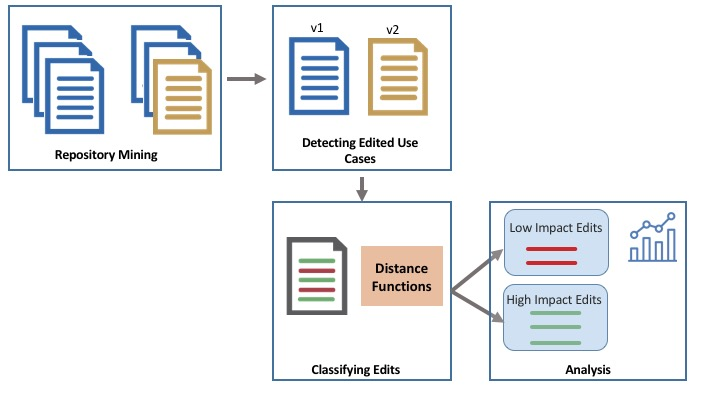
\includegraphics[height=2.3in,width=3.3in]{figs/overview.jpg}
% \caption{Study overview for a single subject.}
% \label{fig:overview}
% \end{figure}

\subsection{Metrics}

To help us evaluate the results, and answer our research questions, we used three of the most well-known metrics for checking binary classifications: \textit{Precision}, which is the rate of relevant instances among the found ones; \textit{Recall}, calculates the rate of relevant retrieved instances over the total of relevant instances; and \textit{Accuracy}, which combines Precision and Recall. These metrics have been used in several software engineering empirical studies (e.g., \citep{nagappan2008influence,hayes2005text, elish2008predicting}). Equations \ref{eq:precision}, \ref{eq:recall} and \ref{eq:acc} present those metrics, where TP refers to the number of cases a distance function classified an edit as low impact and the manual classification confirms it; TN refers to the number of matches regarding high impact edits; FP refers to when the automatic classification reports low impact edits when in fact high impact edits were found; and FN is when the automatic classification reports high impact when in fact should be low impact edits.   

\begin{equation} \label{eq:precision}
Precision = \frac{TP}{TP+FP}
\end{equation}

\begin{equation} \label{eq:recall}
Recall = \frac{TP}{TP+FN}
\end{equation}

\begin{equation} \label{eq:acc}
Accuracy = \frac{TP+TN}{TP+TN+FP+FN}
\end{equation}


\subsection{Results and Discussion} \label{sec:res}

To answer RQ4, we first divided our dataset of use case edits into two (low and high impact edits), according to our manual classification. Then, we ran the distance functions and plotted their results. Figures \ref{fig:bp_dist_l} and \ref{fig:bp_dist_h} show the box-plot visualization of this analysis considering found low (Figure \ref{fig:bp_dist_l}) and high impacts (Figure \ref{fig:bp_dist_h}). As we can see, most low impact edits, in fact, refer to low distance values (median lower than 0.1), for all distance functions. This result gives us evidence that low distance values can relate to low impact edits and, therefore, can be used for predicting low impact changes in MBT suites. On the other hand, we could not find a strong relationship between high impact edits and distance values. Therefore we can answer RQ4 stating that distance functions, in general, can be used to classify low impact.
\\
\\
\noindent
\vspace{2mm} %5mm vertical space
\fbox{\begin{minipage}{23em}
\textbf{RQ4: Can distance functions be used to classify the impact of edits in use case documents?}
Low impact edits are often related to lower distance values. Therefore, distance functions can be used for classifying low impact edits.
\end{minipage}}
\vspace{2mm}


%, but not high impact edits in case documents.

% \begin{figure}[h]
% \centering
% 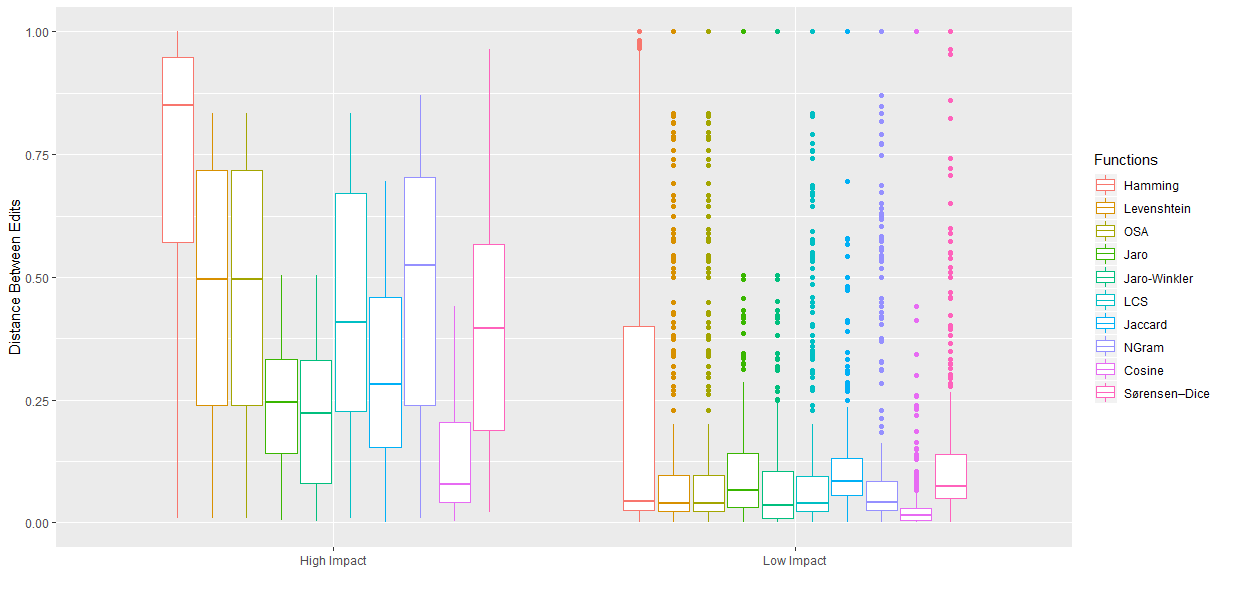
\includegraphics[height=2.3in,width=3.3in]{figs/Boxplot_SAFF_BZT.png}
% \caption{Box-plot for the distance values.}
% \label{fig:bp_dist}
% \end{figure}

\begin{figure}[h]
\centering
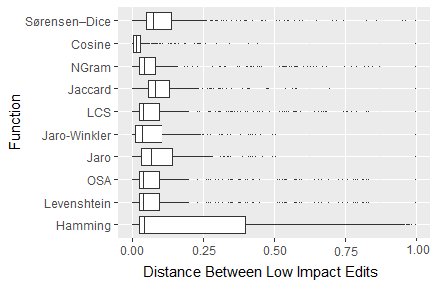
\includegraphics[height=2.3in,width=3.3in]{figs/Boxplot_SAFF_BZT_LOW2.png}
\caption{Box-plot for low impact distance values.}
\label{fig:bp_dist_l}
\end{figure}

\begin{figure}[h]
\centering
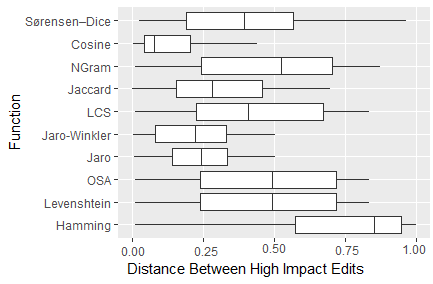
\includegraphics[height=2.3in,width=3.3in]{figs/Boxplot_SAFF_BZT_HIGH2.png}
\caption{Box-plot for high impact distance values.}
\label{fig:bp_dist_h}
\end{figure}

As for automatic classification, we need to define an effective \textit{impact threshold}, for each distance function, we run an exploratory study to find the optimal configuration for using each function. By impact threshold, we mean the distance value for classifying an edit as low or high impact. For instance, consider a defined impact threshold of x\% to be used with function \textit{f}. When analyzing an edit from a specification document, if \textit{f} provides a value lower than \textit{x}, we say the edit is \textit{low impact}, otherwise it is \textit{high impact}. Therefore, we design a study where, for each function, we vary the defined \textit{impact threshold} and we observed how it would impact Precision and Recall. Our goal with this analysis is to identify the more effective configuration for each function. We range the impact threshold between $[0;1]$. 

To find this optimal configuration, we consider the interception point between the Precision and Recall curves, since it reflects a scenario with less mistaken classifications (false positives and false negatives). %Figure 6 presents this analysis for all functions, except Jaccard, while Figure 5 presents the analysis for Jaccard and highlights its best configuration (impact threshold of 0.33).
Figure \ref{fig:best_jaccard} presents the analysis for the Jaccard functions. Its optimal configuration is highlighted (impact threshold of 0.33) --  the green line refers to the Precision curve, the blue line to the Recall curve, and the red circle shows the point both curves meet. Figure \ref{fig:all} presents the analysis for the other functions. 


\begin{figure}[h!] 
\centering 
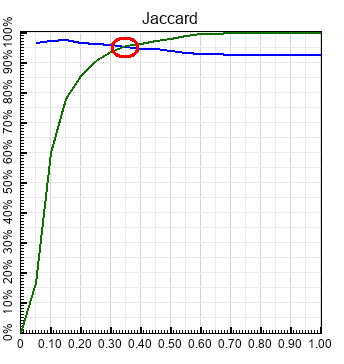
\includegraphics[width=.5\textwidth]{figs/best_Jaccard.png}
\caption{Best impact threshold for the Jaccard function.}
\label{fig:best_jaccard}
\end{figure}


\begin{figure*}[h!] 
\centering 
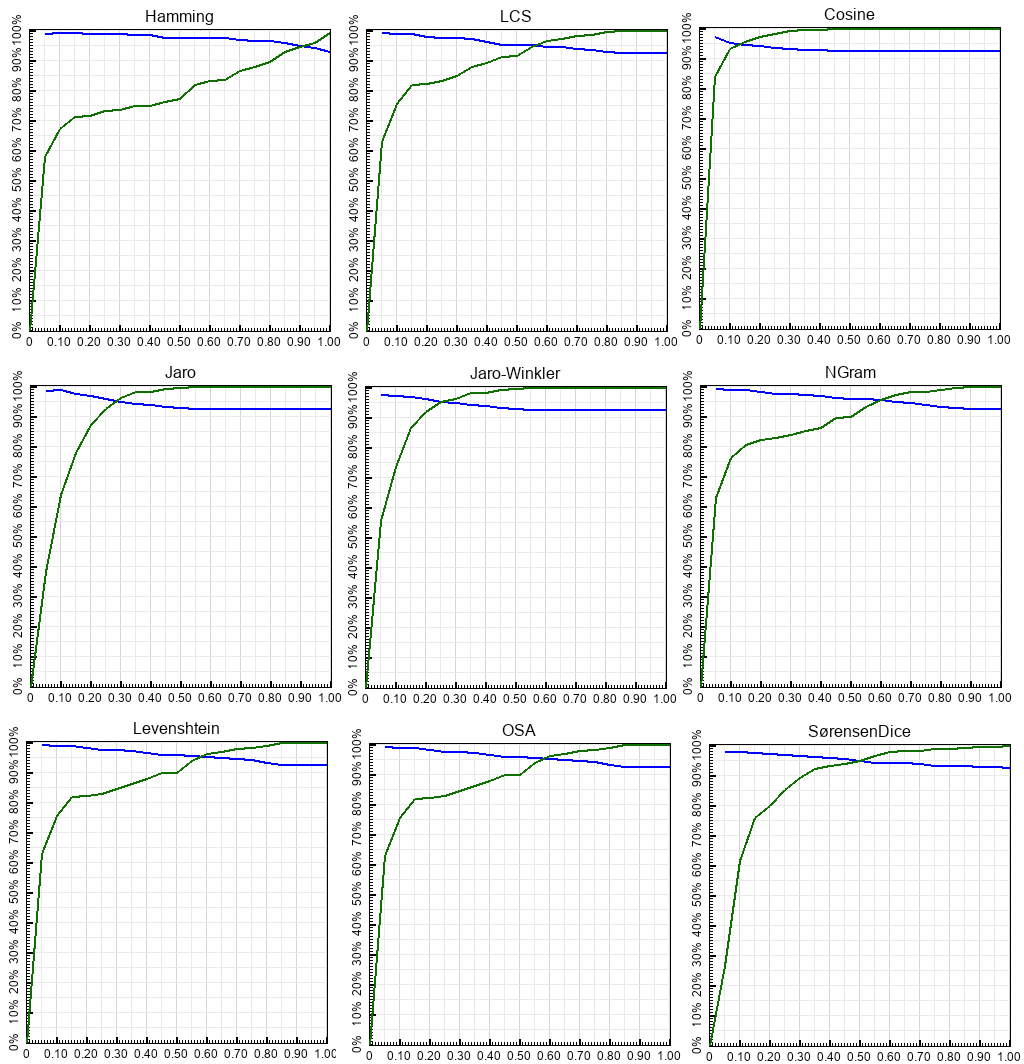
\includegraphics[width=1.0\textwidth]{figs/all.png}
\caption{Exploratory study for precision and recall per distance function.}
\label{fig:all}
\end{figure*}


Table \ref{tab:bestval} presents the optimal configuration for each function and the respective precision, recall, and accuracy values. These results reinforce our evidence to answer RQ4 since all functions presented accuracy values greater than 90\%. Moreover, we can partially answer RQ5, since now we found, considering our dataset, the best configuration for each distance function. To complement our analysis, we went to investigate which function performed the best. First, we run proportion tests considering both the functions all at once and pair-to-pair. Our results show, with 95\% of confidence, could not find any statistical differences among the functions. This means that distance function for automatic classification of edits impact is effective, regardless of the chosen function (RQ5). Therefore, in practice, one can decide which function to use based on convenience aspects (e.g., easier to implement, faster). 

\\
\\
\noindent
\vspace{2mm} %5mm vertical space
\fbox{\begin{minipage}{23em}
\textbf{RQ5: Which distance function presents the best results for classifying edits in use case documents?}
Statistically, all ten distance functions performed similarly when classifying edits from use case documents.
\end{minipage}}

\begin{table}[h]
\caption{Best configuration for each function and respective precision, recall and accuracy values.}
\resizebox{\columnwidth}{!}{%
\begin{tabular}{lcccc}
\multicolumn{1}{c}{\textbf{Function}} & \textbf{\begin{tabular}[c]{@{}c@{}}Impact \\ Threshold\end{tabular}} & \textbf{Precision} & \textbf{Recall} & \textbf{Accuracy} \\
Hamming                               & 0.91                                                                 & 94.59\%            & 94.79\%         & 90.15\%           \\
Levenshtein                           & 0.59                                                                 & 95.22\%            & 95.42\%         & 91.31\%           \\
OSA                                   & 0.59                                                                 & 95.22\%            & 95.42\%         & 91.31\%           \\
Jaro                                  & 0.28                                                                 & 95.01\%            & 95.21\%         & 90.93\%           \\
Jaro-Winkler                          & 0.25                                                                 & 95.21\%            & 95.21\%         & 91.12\%           \\
LCS                                   & 0.55                                                                 & 94.99\%            & 94.79\%         & 90.54\%           \\
Jaccard                               & 0.33                                                                 & 95.22\%            & 95.42\%         & 91.31\%           \\
NGram                                 & 0.58                                                                 & 95.41\%            & 95.21\%         & 91.31\%           \\
Cosine                                & 0.13                                                                 & 95\%               & 95\%            & 90.73\%           \\
Sørensen–Dice                         & 0.47                                                                 & 94.99\%            & 94.79\%         & 90.54\%          
\end{tabular}
}
\label{tab:bestval}
\end{table}